\documentclass[12pt, a4paper, openany, twoside]{book}
\usepackage[italian]{babel}
\usepackage[T1]{fontenc}
\usepackage[utf8]{inputenc}
\usepackage{amsmath} 
\usepackage{xcolor}
\usepackage[margin=1in]{geometry}
\usepackage{hyperref}
\usepackage{graphicx}
\graphicspath{{./img/}}
\usepackage{tikz}
\hypersetup{
    colorlinks=true,
    linkcolor=blue,
    filecolor=magenta,      
    urlcolor=cyan,
}
%usepackage[latin1]{inputenc}
\begin{document}
\fontfamily{cmss}\selectfont
\pagestyle{plain}
\author{DaveRhapsody}
\title {Sistemi Distribuiti}
\date {11 Marzo 2020}
\maketitle
\tableofcontents
\chapter{Introduzione}
Un sistema distribuito è un insieme di componenti hardware e software che 
comunicano tramite scambi di messaggi in rete.
Il concetto di componente è fondamentale, può essere per l'appunto sia hardware
che software.
\paragraph{Nel dettaglio:} E' un sistema di componenti \textbf{autonome},
nel senso che le componenti sono indipendenti tra loro MA concorrono tutte
allo stesso scopo. Per apparire come unico componente occorre generare una
sorta di collaborazione \textbf{SENZA} memoria condivisa.
\paragraph{Autonomia:} Ognuno svolge il proprio compito in modo indipendente
(sia in termini di tempo che dati) da ogni altro. Pertanto occorre che le
componenti siano \textbf{SINCRONIZZATE} (Reti e Sistemi insegna ->).
Questo insieme di nodi appaiono all'utente finale come un unico sistema
\textbf{coerente} senza che lui sappia dove vengono processati (e nemmeno
come) i dati. Il sistema è un blocco unico agli occhi dell'utente MA obv no.
\paragraph{Concetto di trasparenza:} Il livello di trasparenza lo si decide 
in fase di progettazione del sistema, fondamentalmente è il livello tale per 
cui l'utente sappia come vengono processati i dati, e cosa e come viene
eseguito dal sistema. (Un sistema trasparente, è un sistema che ti fa
vedere vita, morte, miracoli, luci, coriandoli, sassi e Babbo Natale).
\section{Caratteristiche fondamentali}
\begin{itemize}
	\item Non c'è memoria condivisa
	\item L'esecuzione è concorrente (allo stesso istante)
	\item Non ci sono stati del processo o della memoria, ogni nodo è a sè un
	processo!
	\item NON C'E' UN CLOCK GLOBALE, niente scheduling. controllo (globale),
	si fa tutto per scambio di messaggi
	\item Non esiste un fallimento globale ma un fallimento della singola
	componente. 
	\paragraph{Sistemi Realtime:} Noi non utilizziamo questo genere di 
	dispositivi, studiamo e prendiamo in esame dispositivi best-effort
	\item Architetture software
\end{itemize}
\section{Architetture software}
E' la struttura del sistema, di come sono organizzate le componenti, quali
sono i protocolli, le interfacce, etc.
\begin{itemize}
	\item Architetture a Livelli (tier)
	\item Architetture a oggetti
	\item Architetture centrate sui dati
	\item Architetture event-based (ajax)
\end{itemize}
\subsection{Stratificazione}
L'idea è formare degli strati di complessità, fondamentalmente nulla vieta di 
fare tutto a livello application, lì si impreca per davvero, ma soprattutto
non ci sarebbe una specializzazione. Il motto è "Fai una cosa, ma falla bene".
\section{Tipi di sistemi operativi}
In base al tipo ho un livello diverso di trasparenza
\begin{itemize}
	\item DOS: Distributed OS
	\item NOS: Network OS: L'OS ti dà delle librerie e supporti per supportare
	delle applicazioni MA non nasconde le comunicazioni tra le varie applicazioni.
	\item Middleware: Hai un insieme di sistemi di rete che forniscono primitive
	per sostenere comunicazione tra sistemi E costruirci delle logiche che 
	consentano di vedere questo come unico sistema (Sì, il middleware è 
	a sua volta un'applicazione distribuita)
	\section{Servizi del middleware}
	\begin{itemize}
		\item Naming
		\item Accesso trasparente
		\item Persisenza: avviene una memorizzazione di dati persistente
		\item Transazioni distribuite: Va garantita la consistenza dei dati
		\item Sicurezza dei dati: integrità computazionali
	\end{itemize}
	\paragraph{Riporto il riassunto presente nelle slides}  
	\begin{center}
	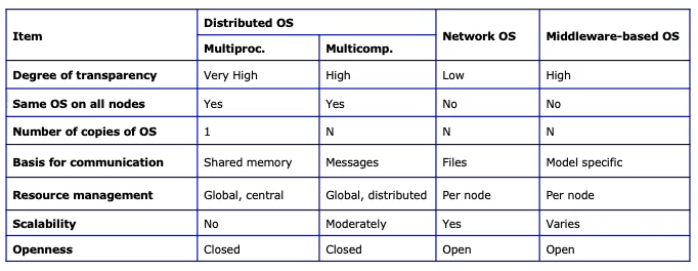
\includegraphics[width=0.75\textwidth]{1.png}
	\end{center}
\end{itemize}
\chapter{Modello Client-Server}
E' un'interazione basata su richiesta-risposta tra una componente e 
l'altra.
\paragraph{Funzionamento:}
\begin{enumerate}
	\item Client invia la request
	\item Server la riceve, client aspetta
	\item Server elabora
	\item Server risponde alla richiesta
\end{enumerate}
Quando client aspetta, quest'ultimo è in standby, in attesa, fermo, inchiodato.
Il server si attiva ad ogni richiesta che arriva. Richiesta e risposta hanno
un tempo ovviamente proprio, che deriva dalla rete di riferimento, chiaramente
se si fa tutto sulla stessa macchina si parla di microsecondi.
\paragraph{Osservazione:} Un dispositivo è sia client che server, può essere
sia uno che l'altro.
\paragraph{Tipi di accesso:}
\begin{itemize}
	\item Accesso a server multipli (nel senso che sono duplicati i server)
	\item Accesso via proxy
\end{itemize}
\section{Problemi dei Sistemi Distribuiti}
\begin{itemize}
	\item Identificazione della controparte: Identifico la risorsa, tipo con
	address etc.
	\item Accesso alla controparte: Dove accedo? Chi è il mio access point
	\item Comunicazione 1: Definisco il formato dei messaggi scambiati
	\item Comunicazione 2: Capisco il contenuto del messaggio in seguito 
	all'estrazione
	\paragraph{Esempio:} I tipi per i dati, che specificano un insieme 
	di valori ed operazioni fattibili su un determinato dato.
\end{itemize}
\section{Trasparenza}
Significa nascondere all'utente \textbf{come} viene ottenuto un determinato
risultato. E' per intenderci ciò che salva coloro che programmano tutto nel 
main.
Come si fa?
\begin{itemize}
	\item \textbf{Naming}: non mi connetto per indirizzo IP ma per indirizzo web, link.
	\item \textbf{Accesso trasparente}: Come accedo in maniera trasparente? Anche qui
	nomi simbolici, qualcosa che non mi faccia capire la locazione della 
	controparte
	\item \textbf{Location Trasparency}: Hai una stampante a casa e devi stampare una foto
	di gattini? Ti serve sapere dove si trova, non puoi cercare a caso su google,
	quindi devi sapere fisicamente dove hai la stampante. Invece se ti serve
	una calcolatrice online tipo wolfram alpha, digiti l'equazione, la risolve,
	ma tu non sai una bega di dove è stata risolta.
	\item \textbf{Relocation o trasparenza mobile}: Posso spostare le risorse mentre le
	uso (Cellulari, dispositivi wifi, ci siamo capiti).
	\item \textbf{Migrazione}: Posso spostare un sito web da un pc del 91 ad un pc del 
	2020, il servizio quello è, cambierà la velocità (tempi di elaborazione
	+ request + response)
	\item \textbf{Replicazione}: Hai una serie di server identici, tu ti connetti ad uno
	o l'altro, cambia niente
	\item \textbf{Concorrenza}: In più utenti accediamo allo stesso servizio (spotify)
	\item \textbf{Trasparenza del fallimento}: Ciò che resta dopo un fallimento di una
	componente deve colmare i danni di una componente morta.
	\item \textbf{Persistenza}: Non mi accorgo di quando un sistema è riavviato o no
\end{itemize}
In alcuni casi è impossibile nascondere un fail o lo stato di una applicazione,
se ti crasha Word, vedi che ti è crashato Word, quindi in qualche modo 
va comunicato all'utente "Ueh, fa schifo Uord, usa OpeNoFFiSsszsxxs". Ma
tra l'altro non sempre è utile nascondere, prendete l'esempio di prima della
stampante. 
\section{Separazione tra interfaccia e realizzazione}
Costruisco un'astrazione logica che nasconde i dettagli implementativi
di ciò che sta diestro. Ogni componente pubblica il What cioè COSA fa, ma non
ti spara fuori anche l'HOW, cioè COME lo fa, è il concetto di information
hiding di Java.
\paragraph{Esempio:}
Gestione delle stringhe nei vari linguaggi. Una stringa è una concatenazione
di caratteri, la gestione di append, copy, concat etc. sono how, il 
risultato finale è il what
\section{Politiche versus mechanism}
Un Sistema distribuito è composto da.. Va beh avete capito. Progressivamente
si va verso un unico enorme (utopico) sistema complesso organizzato con delle
policy stabilite. 
Le politiche banalmente sono una serie di regole ad esempio prendete il context
switch di Unix. 
\begin{itemize}
	\item Il CS è un meccanismo
	\item Il Round Robin invece è la policy di come è gestito un comportamento	
\end{itemize}
\section{Concetto di protocollo}
Un protocollo è un insieme di regole che definiscono un formato, l'ordine,
payload, operazioni da compiere alla ricezione od all'invio di un 
messaggio.
\chapter{Le Socket}
\paragraph{Cos'è?} Una socket è un'interfaccia tra il sistema operativo ed un 
processo su di esso eseguito, quindi un programma in stato di esecuzione.
\textbf{Come?} Fondamentalmente dati due processi, la socket è colei in grado di
metterli in comunicazione inviando o leggendo dati.
\section{Aspetti critici}
\subsection{Gestione del ciclo di vita di client e server}
Quando si attiva e/o disattiva uno dei due, chi la gestisce è il middleware, 
oppure può essere manuale
\subsection{Identificazione ed accesso al server}
Un client per accedere ad un server deve conoscerne l'indirizzo ed una serie di
informazioni che consentano di raggiungerlo.
\paragraph{Come fa un client a conoscere l'indirizzo server?} Ha diverse alternative
\begin{itemize}
	\item Inserisce nel codice del client l'indirizzo del server espresso
	come costante (Il client di un servizio bancario)
	\item Si chiede all'utente di inserire l'indirizzo (E' quello tipico di 
	browser e simili)
	\item Si può utilizzare un \textbf{name server} o si attinge da un repository
	da cui il client può acquisire informazioni necessarie
	\item Si adotta un protocollo differente per individuare il server (ad 
	esempio il DHCP)
\end{itemize}
\subsection{Comunicazione client server}
Quali sono le primitive disponibili? Quali sono le modalità di comunicazione?
\subsection{Ripartizione dei compiti client e server}
Dipendentemente dal tipo di applicazione si decide chi fa cosa, quali compiti
spettano al server, quali al client. Come si decide? Si deve fare un'analisi
dei rischi in fatto di sicurezza, prestazioni etc.
\section{Soluzioni agli aspetti critici}
\begin{enumerate}
	\item Si identifica la controparte, tramite il naming, ogni host avrà un nome,
	si fa riferimento ad un indirizzo ed una porta
	\item Per accedere alla controparte servirà accedere all'indirizzo:porta,
	usando direttamente l'indirizzo IP (access point)
	\item Comunicazione 1: (Protocolli) Stream di byte
	\item Comunicazione 2: (Sintassi e semantica) Metodo di interpretazione dei 
	flussi di byte 
\end{enumerate}
Il livello di trasparenza è basso poichè è il programmatore che deve preoccuparsi
di queste problematiche
\section{Comunicazione via socket}
Le comunicazioni in TCP/IP avvengono tramite flussi di byte in seguito ad una
connessione esplicita con systemcall read/write
\paragraph{Perchè?} Perchè sono due funzioni sospensive, ovvero bloccano il processo
finchè non è raggiunto il completamento dell'operazione e soprattutto viene
utilizzato un buffer per garantire flessibilità
\paragraph{Come funziona?}
\begin{enumerate}
	\item Il server richiede di aprire un canale in ascolto (Socket bind)
	\item Il client con una socket crea un canale analogo, senza una bind, ma 
	con stesso effetto finale
	\item Il client invia la richiesta, il cui formato è stabilito dal livello
	di trasporto
	\item Il server crea un secondo canale di comunicazione che sarebbe l'accept,
	quindi avviene l'handshake, poi si procede con il trasferimento
\end{enumerate}
Non si comunica sulla stessa socket poichè da una socket o si entra o si esce,
non si possono fare entrambe le cose.
\chapter{Tipi di comunicazione}
Ci sono fondamentalmente diversi tipi di comunicazione. Il primo tipo è la 
comunicazione orientata ai messaggi. Per capire meglio come funzioni quest'ultima
si fa riferimento all'architettura del Web, ma prima definiamo la comunicazione
orientata ai messaggi.
\section{Comunicazione orientata ai messaggi}
Come accennato prima, questo tipo di comunicazione prevede lo scambio di messaggi,
generalmente uno richiesta e uno risposta, ed è tutto gestito e controllato da 
dei protocolli.
\subsection{Protocolli}
Un protocollo è un insieme di regole atte a stabilire formato, ordine di invio e
ricezione, dispositivi, tipi per i dati ed azioni da eseguire in invio e ricezione
di un messaggio
\paragraph{Alcuni esempi di protocolli:} HTTP, SFTP, SMTP, FTP, verranno definiti
in seguito.
\subsection{Protocollo HTTP}
Il web (dopo si vedrà come) lavora prevalentemente con HTTP (hypertext transfer
protocol), quindi tramite 
scambio di HTTP requests e responses tra client e server, è fondamentalmente
il protocollo in grado di trasferire dell'ipertesto.
\paragraph{Cosa c'è alla base di HTTP?} Livello transport: TCP, nello specifico
instanzia una socket sulla porta 80, il server accetta la connessione (Handshake
a 3 vie) e si effettuano gli scambi
\paragraph{E' un protocollo stateless: } Il server non si ricorda delle richieste
precedenti, quindi una richiesta deve avere tutte le informazioni richieste per
l'esecuzione. Ci sono altri protocolli che mantengono però l'informazione.
\paragraph{Formato dei messaggi HTTP: } Request e response hanno la stessa
struttura: 
\begin{center}
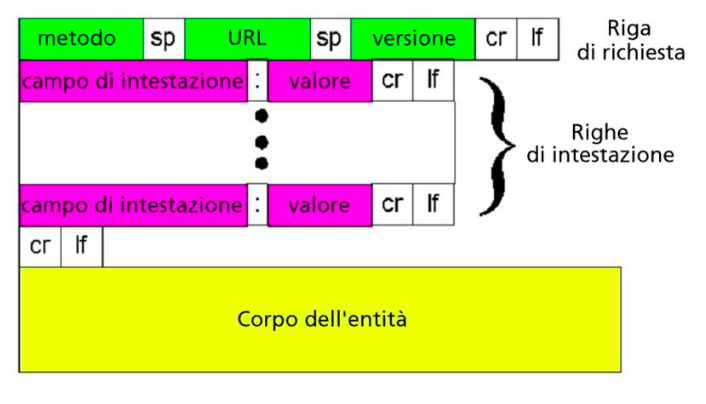
\includegraphics[width=0.75\textwidth]{2}
\end{center}
\paragraph{Esempio di messaggio HTTP request:}
\begin{center}
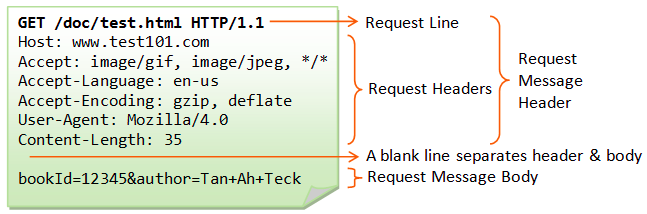
\includegraphics[width=0.75\textwidth]{3}
\end{center}
\subsection{Metodi per effettuare HTTP requests}
Sono fondamentalmente 3:
\paragraph{Metodo GET:} Restituisce una rappresentazione di una risorsa, include
un eventuale input in coda alla URL della risorsa, l'esecuzione non ha effetti sul server
ed è gestible da una cache del client
\subparagraph{Specificazione: }Una get può essere condizionale, per evitare di 
inviare roba che il client ha già nella cache. Ad esempio ci puoi mettere un
if-modified-since: data che banalmente non trasferisce nulla se l'ultima modifica
è entro una certa data. 
\subparagraph{E la risposta?} Il server dà risposta vuota se l'oggetto è aggiornato.
HTTP/1.0 304 Not Modified 		
\subparagraph{Uso tipico:} Ottenere dati in formato di pagine html e immagini
\paragraph{Metodo POST:} Comunica dei dati che vengono elaborati lato SERVER o
crea una risorsa subordinatta all'URL, inoltre non è idempotente, ogni esecuzione
ha un effetto diverso, e la risposta non è gestibile con una cache lato client.
E' usata per gestire i FORM o modificare i DB
\paragraph{Metodo HEAD:} Molto simile alla GET ma restituisce solo l'HEAD della
pagina web, si usa spesso in fase di debug.
\paragraph{Ecco una tabella riassuntiva dei metodi HTTP:} 
\begin{center}
	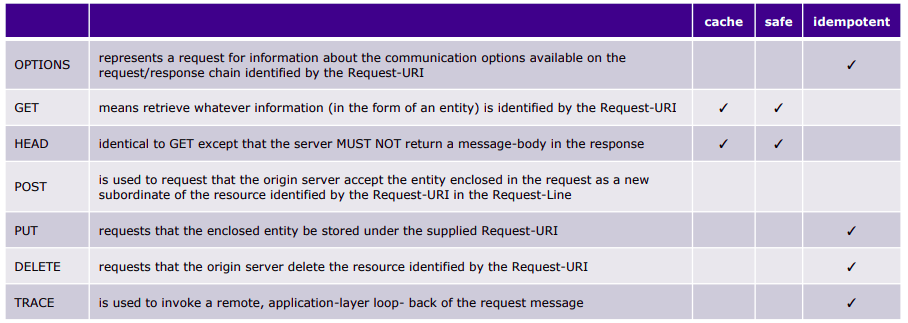
\includegraphics[width=0.75\textwidth]{4}
\end{center}	
\paragraph{Formato di una HTTP response:}
\begin{center}
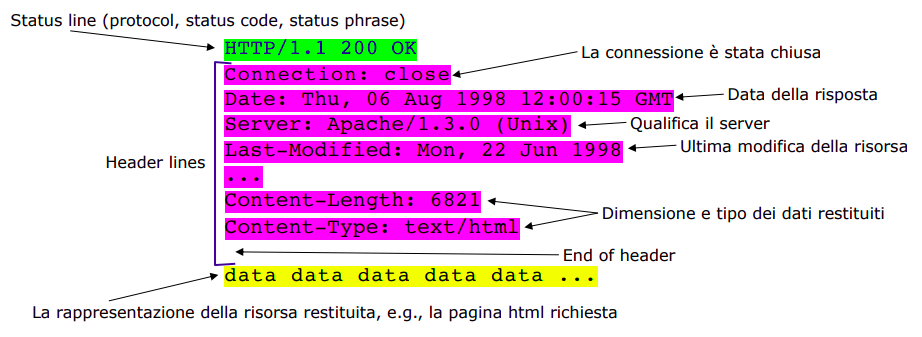
\includegraphics[width=0.75\textwidth]{5}
\end{center}
\subsection{I tipi MIME}
Nella parte del web si vedrà una specificazione di questi, fodamentalmente 
MIME significa Multipurpose Internet Mail Extension, qualifica i dati
via Internet (in HTTP, qualifica il tipo dei dati del body)
\paragraph{Quali sono questi tipi? }Testo, immagini, video, audio, dati che devono
essere processati da un'applicazione prima di esser visibili
\subsection{I cookie}
Un cookie serve per legare più richieste in modo da associare un ID alla conversazione.
Il client manda al server un cookie, che è un numerello, ed il server saprà
chi è che parla ogni volta che riceve quel cookie per gli accessi positivi.
\paragraph{Come vien controllato? }Il server autentica ogni cookie, traccia
le preferenze dell'utente e la sessione di lavoro (Sì, esatto, quella roba dei
cookie che si legge in ogni sito serve a questo)
\paragraph{Come controllo l'accesso ai documenti lato server?} Consideriamo che
HTTP è stateless, il client deve autenticare ogni richiesta, perciò molto
semplicemente il client manda login e password nell'header del messaggio, e 
per evitarsi che l'utente li digiti ogni volta, se li salva. Not bad!
\section{Comunicazione orientata allo stream}
Questa cosa è stata menzionata nella parte relativa al livello di trasporto
del modello TCP/IP, fondamentalmente è la differenza tra TCP e UDP. TCP numera
ogni elemento della sequenza, garantisce la correttezza dell'informazione, 
l'ordine, e l'integrità. Invece UDP di questo non si cura.
\paragraph{E al lato applicativo? } L'applicazione invia i messaggi come stream 
di byte al livello di trasporto, e poi leggerà i byte dal trasporto ricostruendo
i messaggi. Ma non si cura di ciò che c'è sotto
\section{Architettura del web}
Il web supporta l'interazione tra client e server mediante HTTP, e a seconda del
fatto che un host sia client o server cambierà il tipo di messaggio che invia
(o riceve). 
\begin{itemize}
	\item Se si tratta di un \textbf{Server} riceverà delle HTTP \textbf{Requests}
	\item Se si tratta di un \textbf{Client} riceverà delle HTTP \textbf{Response}
\end{itemize}
Client e server sono rispettivamente rappresentati da:
\begin{itemize}
	\item Client: un Browser, od un User-Agent
	\item Server: un web server o HTTP server
\end{itemize}
\section{Tipi di comunicazione}
Esistono diversi tipi di comunicazione:
\begin{enumerate}
	\item Comunicazione sincrona o asincrona
	\item Comunicazione transiente (se il destinatario non c'è, i dati sono 
	scartati)
	\item Comunicazione persistente: Il middleware memorizza i dati fino alla consegna
	del messaggio, non serve che i processi siano in esecuzione prima e dopo l'invio.
\end{enumerate}
\subsection{Comunicazione persistente}
Un messaggio persistente può esser sia sincrono che asincrono, la differenza nel fatto che
nel caso dell'asincrono, dati A e B che voglion comunicare:
\begin{enumerate}
	\item A invia un messaggio e continua a fare il suo
	\item B si sveglia ad un certo punto, e riceve il messaggio
\end{enumerate}
Mentre nel caso il messaggio è sincrono
\begin{enumerate}
	\item A invia un messaggio a B e si ferma ad aspettare
	\item B non è in esecuzione ma il messaggio verrà salvato in un buffer
	che leggerà al risveglio
	\item A riceve l'ok dell'inserimento del dato in quel buffer, e torna a fare il suo
	\item B si sveglia, e riceve il messaggio
\end{enumerate}
Nel caso di una comunicazione asincrona transiente:
\begin{enumerate}
	\item A manda il messaggio e fa il suo
	\item B riceverà solo se è in esecuzione
\end{enumerate}
Nel caso invece la comunicazione è sincrona A invia e aspetta che b riceva e risponda.
Invece per le comunicazioni transienti delivery-based si ha che:
\begin{enumerate}
	\item A invia una richiesta e aspetta
	\item B si sta facendo i cazzi suoi da acceso, riceve, risponde con comodo
	\item A riparte da quando riceve l'accepted, e poi B processa la sua richiesta
\end{enumerate}
Invece nel caso sia una response-based..
\begin{enumerate}
	\item A invia il messaggio, e non solo aspetta che B risponda, ma aspetta
	che B finisca di processare, producendo un Sent-request delay.
\end{enumerate}
\subsection{Web browser}
Considerando il lato client si ha questo software che consente di visualizzare
le pagine web, è detto \textbf{User-Agent}, fondamentalmente ciò che fa un 
browser è \textbf{interpretare} un codice di mark up (HTML, ad esempio), che
sarebbe una pagina web, e successivamente visualizzarlo (in forma di ipertesto)
\paragraph{Mh.. Manca qualcosa:} Assieme all'HTML (che delinea la grafica) un
browser consente (soprattutto se $browser \neq Internet-Explorer$) molta più
roba, dalla multimedialità, ai feed RSS, ai file XML, Json etc. 
\subsection{La pagina web}
Come accennato nella sottosezione precedente, si hanno delle vere e proprie 
pagine web, che fondamentalmente sono dei file, dei documenti, costituiti da
un certo insieme di oggetti, o \textbf{risorse}.
\paragraph{Definizione di risorsa:} Una risorsa è una \textbf{sequenza di dati}
\textbf{identificata da un URL}, che per intenderci è un indirizzo univoco. 
Questo insieme di dati risiede su \textbf{memoria di massa} e quindi è per 
semplificarci la vita un \textbf{file}. 
\paragraph{Okay, che file abbiamo?} La maggior parte delle pagine web ha almeno
una riga di HTML (Hypertext Markup Language), anche solo per definire i contenuti
testuali e qualche elemento grafico
\paragraph{E il web server?} Il web server è l'applicativo che ha il compito di
gestire quei famosi file, e soprattutto che li rende disponibili ai client (Se
c'è un mondo dietro ai browser, per fare a gara tra quale è il migliore, c'è 
anche lato server. Sì.)
\subsection{L'URL}
Un URL (Uniform Resource Locator) identifica un oggetto nella rete, ma non è questo
il lato più importante
\paragraph{Un URL specifica il protocollo con cui si possono interpretare i dati}.
\paragraph{Come è composto?} E' composto da 5 componenti principali:
\begin{enumerate}
	\item Nome del protocollo (sftp, http, https, ftp, smtp etc.)
	\item Indirizzo dell'host (IP address)
	\item Porta di destinazione 
	\item Percorso file nell'host
	\item Risorsa
\end{enumerate}
\paragraph{Esempio: accedi in ftp a 192.168.50.5 al percorso /media/hdd e 
prendi il file prova.txt} ftp://192.168.50.5:21/media/hdd/prova.txt
\subsection{Ipertesto}
Per tre volte si è menzionato l'\textbf{ipertesto}, ma cosa sarebbe? Fondamentalmente
è un insieme di testi o pagine leggiili tramite un'interfaccia elettronica. 
Funzionano tramite hyperlink, o anche solo link.
\paragraph{E che fanno i link?} Costituiscono una rete raggiata, o incrociata di
informazioni organizzate su citeri paritetici o gerarchici (I menù, per capirci)
\subsection{Linguaggi del web}
I dati testuali si esprimono con linguaggi standard (HTML, XML e JSON),
rispettivamente descrivono: Struttura contenuti (HTML) e struttura dei dati (JSON, XML)
\paragraph{E i dati non testuali?} Esiste una tecnica di encoding detta MIME che
consente di definire il formato dei contenuti non testuali (video, audio, etc.)
\paragraph{Ma gli script?} Lasciati in disparte fin dal principio, questi 
sono essenziali, consentono la creazione di pagine web \textbf{dinamiche}.
Alcuni dei più famosi: VBScript, PHP, JavaScript, Adobe Flash etc.
\chapter{HTML, DOM, CSS, JAVASCRIPT}
Sono tutti linguaggi, sebbene non tutti dello stesso tipo. Di fatto Javascript è
un linguaggio di programmazione (In questo caso interpretato) mentre per quanto
riguarda HTML e CSS si fa riferimento a linguaggi di Markup
\section{Linguaggi di markup}
\paragraph{Cosa sono?} In modo semplificativo, sono linguaggi che dicono 
all'interprete come rappresentare graficamente un foglio, o una pagina (in questo
caso web). 
\paragraph{Solo per pagine web?} No, questo documento è stato scritto in LaTeX, 
che è un linguaggio di MarkUp per documenti PDF, però non è solo questa la differenza.
Infatti LaTeX è compilato, mentre HTML, Markdown e simili sono tutti interpretati.
\paragraph{Chi è l'interprete di HTML+CSS?} Qualsiasi browser, addirittura anche
Internet Explorer (Con un quarto d'ora di ritardo, ma c'è).
\subsection{HTML}
Hypertext Markup Language, per l'appunto, linguaggio di markup per strutturare contenuti
web (L'ipertesto). Quando si è di fronte ad una pagina web, 9/10 è scritta, o 
contiene, del codice in HTML
\subsection{CSS}
Cascading Style Sheets, è un linguaggio di supporto all'HTML che invece serve per
dare uno stile di presentazione ai contenuti, quindi fondamentalmente è tipo una
libreria di quelle che si importa in Java o C. Da solo non serve a niente, ma 
integrandolo con HTML, porta a pagine carine
\paragraph{Diversi stylesheet:} Ne esistono diversi, per l'appunto \\
\begin{itemize}
	\item L'autore della pagina in genere ne specifica uno, o anche più di uno
	\item Il browser ne ha uno solo, o un vero css, oppure uno simulato nel codice
	del browser
	\item Il lettore, l'utente del browser, ne può definire uno personale per
	modificare la propria esperienza d'uso.
\end{itemize}
\subsection{DOM}
Document Object Model, è un'interfaccia neutrale rispetto al linguaggio di programmazione,
è fondamentalmente quello che consente ad una pagina web di essere dinamica ed 
avere del codice sotto che funziona. Form, elenchi, quella roba lì.
\paragraph{Precisazioni:} Usare HTML e CSS serve per fare in modo che contenitore
e contenuto siano indipendenti l'un dall'altro, la separazione dei concetti infatti
è ormai d'obbligo in informatica, PERO' lo stile può avere un coupling, un legame
con il contenuto. \\ \\
Il browser infatti non è un lettore di pagine scritte in HTML e morta lì, ma è un
ambiente di sviluppo che fornisce un numero enorme di funzionalità. Se premete
su una qualunque pagina F12 capirete meglio il concetto.
\chapter{Servlet e Applicazioni Web}
Prima di capire cos'è una servlet serve dare una veloce spiegazione di come funziona
un'applicazione web. \\ \\
Come spiegato in qualche precedente capitolo, tutto è basato su un'architettura 
client-server, quindi ci sarà un Web Client (Browser) ed un web server (Apache
o simili).
\paragraph{Come si passa dal Web alle applicazioni?} Partendo dal fato che il web
supporta l'interazione tra client e server via HTTP, il server avrà un programma 
che si chiama Application Server (E' UN SOFTWARE, NON HARDWARE) che è caratterizzato
dal protocollo di interazione con il Web Server stesso. L'interazione con il client
è infatti tutta in HTTP.
\paragraph{Cosa accade lato server?} Ogni calcolo, ogni computazione, viene 
svolta dal server, e può avvenire sia da scriptini che da programmi compilati.
Nel caso di software compilati ciò che accade è che il server invoca l'eseguibile
(Partendo dalla richiesta del client). 
\paragraph{Come vengono eseguiti gli script?} Il Web Server ha un motore in grado
di intepretare il linguaggio di scripting di riferimento, quello richiesto, per intenderci
\section{Sigle da sapere}
\begin{enumerate}
	\item URL: Uniform resource locator, definisce un naming globale, un modo per 
	tracciare le cose
	\item CGI: Content Gateway Interface, permette al server di attivare un 
	programma, passargli le richieste e i parametri dal client, e recuperare 
	una risposta
	\paragraph{Che vantaggi ci sono?}
	\begin{itemize}
		\item Ti devi programmare solo le logiche
		\item Hai un modello di applicazioni conformi al modello del linguaggio
		\item Semplice, riproducibile ovunque, manutenibile in modo agevole
	\end{itemize}
	\section{Servlet}
	Finalmente si arriva alle Servlet. Che sono? Sono applicazioni Java che si 
	trovano sul server. E' un componente che il server gestisce in modo automatico
	da un engine, oppure da un container. 
	Dalle slide c'era qualche esempio di come si costruiscono e usano.
	\section{Remote Procedure Call}
\end{enumerate}






















    

























\end{document}